\subsection{Unwürdiger Abschied als Chorregent}

\hypertarget{RefHeadingToc100333737}{}Ähnlich große Wellen wie die
Entlassung des Chorregenten Max Rauscher im Jahr 1927 schlug 1953
August Högns Ausscheiden als Kirchenchorleiter. Dem Chorleiterwechsel
ging ein Pfarrerwechsel voraus. Am 17. Februar 1953 verstarb Pfarrer
Jakob Bauer. \footnote{Reicheneder-Chronik, Seelsorger, Blatt III/14
(4) Vorderseite} Der neue Pfarrherr Franz Seraph Reicheneder wurde am
26. Mai 1953 in Ruhmannsfelden empfangen und am 14. Juni\footnote{
Reicheneder-Chronik, Seelsorger, Blatt III/15 (1) Vorderseite}
schließlich feierlich mit Högns „Josephi“-Messe installiert.\footnote{
Dokument Nr. 41, Zeitungsartikel aus dem Viechtacher Bayerwald-Boten,
15.6.1953} August Högn wollte eigentlich bei Antritt des neuen Pfarrers
seinen Rücktritt als Chorregent und Organist bekannt geben, doch der
neue Pfarrer lehnte sein Ersuchen anstandsgemäß ebenso wie vor einiger
Zeit Pfarrer Jakob Bauer und in der Übergangszeit Pfarrprovisor Georg
Huber ab. \footnote{Dokument Nr. 18, Brief von August Högn an Pfarrer
Reicheneder, 25.1.1954} August Högns Rücktrittsabsichten sprachen sich
sogar herum, sodass Josef Brunner – er war während der Kriegszeit
Aushilfsorganist in Ruhmannsfelden – eine Bewerbung für die
möglicherweise frei werdende Chorregentenstelle bei der
Kirchenverwaltung Ruhmannsfelden einreichte. \footnote{Dokument Nr. 17,
Brief von Josef Brunner an Kirchenverwaltung, 29.4.1953}

\begin{center}
\begin{minipage}{4.032cm}
\begin{flushleft}
\tablefirsthead{}
\tablehead{}
\tabletail{}
\tablelasttail{}
\begin{supertabular}{m{3.832cm}}

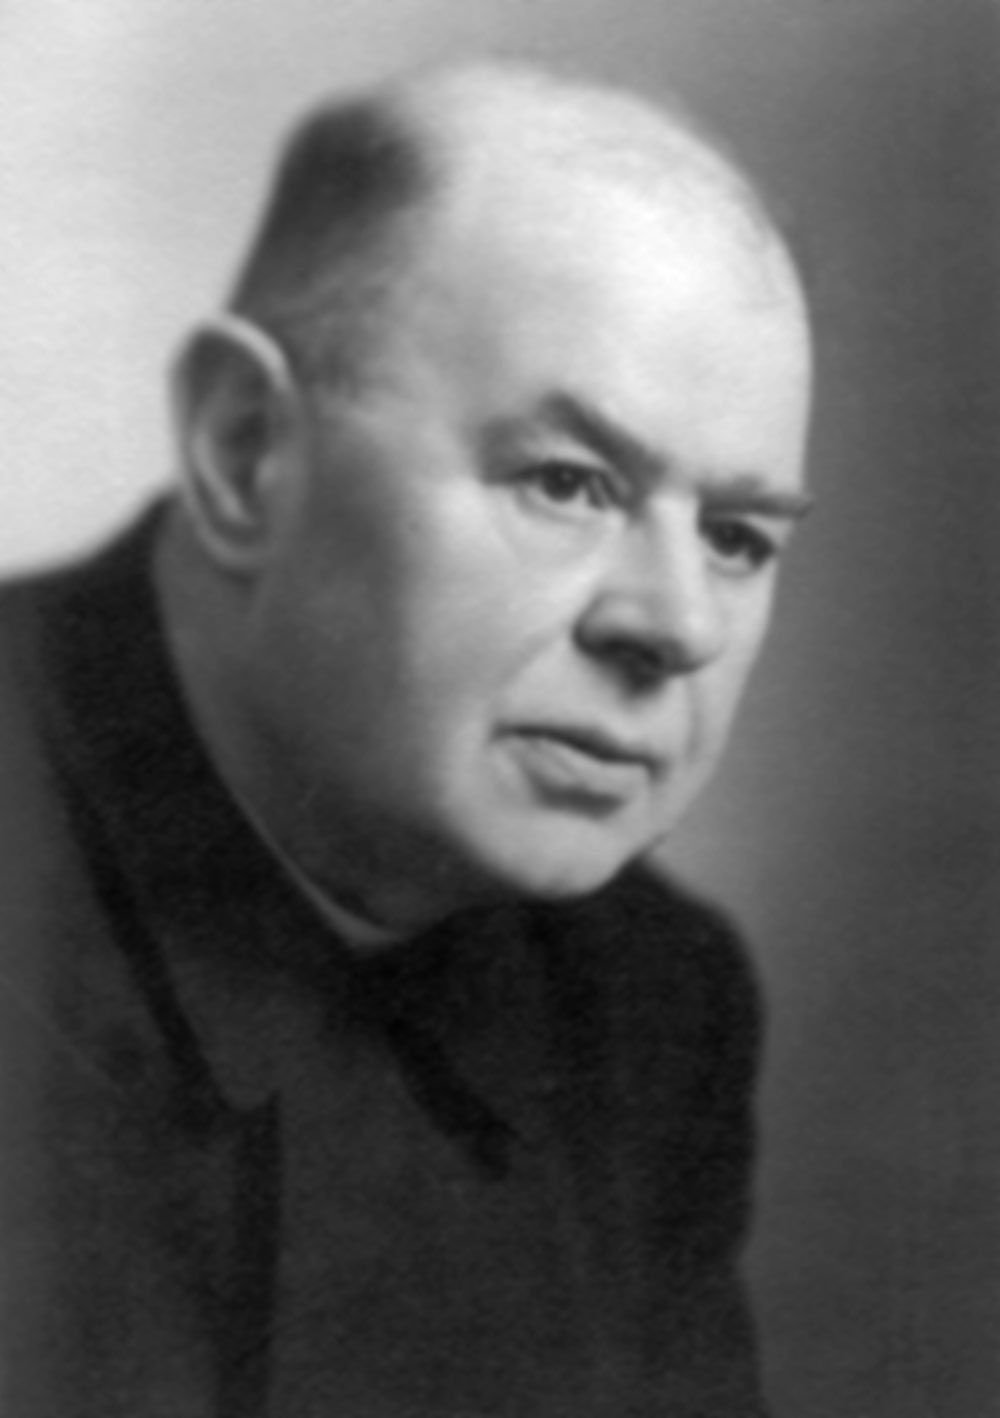
\includegraphics[width=3.651cm,height=5.177cm]{pictures/zulassungsarbeit-img046.jpg}

Abb. \stepcounter{Abb}{\theAbb}: Jakob Bauer\\
\end{supertabular}
\end{flushleft}
\end{minipage}
\end{center}
Umso verwunderlicher ist die Dramatik wie sich Högns Ausscheiden als
Chorregent dann tatsächlich vollzog: Nachdem Högns Bitte um Rücktritt
von Pfarrer Reicheneder abgelehnt wurde, scheint Högn weiterhin mit
einer längerfristigen Dienstzeit als Chorregent und Organist gerechnet
zu haben, sonst hätte er nicht schon 1953 zwei Marienlieder zum
marianischen Jahr 1954 komponiert. Reicheneder hingegen, von Högns
Amtsmüdigkeit überzeugt, war wahrscheinlich davon ausgegangen, dass der
75-jährige Högn bald abdankt würde. \footnote{Interview Nr. 24, Johann
Glasschröder, 28.12.2004, Absatz 48} Vielleicht hatte er auch schon
deswegen seiner von vorneherein favorisierter Nachfolgerin Maria
Reisinger eine baldige Anstellung in Aussicht gestellt. Maria
Reisinger, ein Waisenkind, war Reicheneders Ziehtochter, um deren
Ausbildung sich Reichender gekümmert hatte.

Mit Sicherheit hat Reicheneder die Ablehnung des Rücktrittsgesuchs aus
folgenden zwei Gründen bereut: Zum einem war für seine Ziehtochter
keine Anstellung in absehbarer Zeit greifbar, zum anderen leisteten zum
damaligem Zeitpunkt Högn und sein Chor äußerst schlechte Darbietungen.
Die Aufführung der „Josephi“-Messe durch den
\zitat{„klangvollen Chor“}
\footnote{Dokument Nr. 41, Zeitungsartikel aus dem Viechtacher
Bayerwald-Boten, 15.6.1953} zu Reicheneders Installation war nicht
repräsentativ für den alltäglichen Kirchenmusikbetrieb, da hier viele
Aushilfen mitwirkten \footnote{Interview Nr. 24, Johann Glasschröder,
28.12.2004, Absatz 44} und hatte möglicherweise bei Reicheneder ein
falschen Eindruck hinterlassen.

\begin{flushleft}
\tablefirsthead{}
\tablehead{}
\tabletail{}
\tablelasttail{}
\begin{supertabular}{m{3.5939999cm}m{4.361cm}m{4.123cm}m{3.3769999cm}}

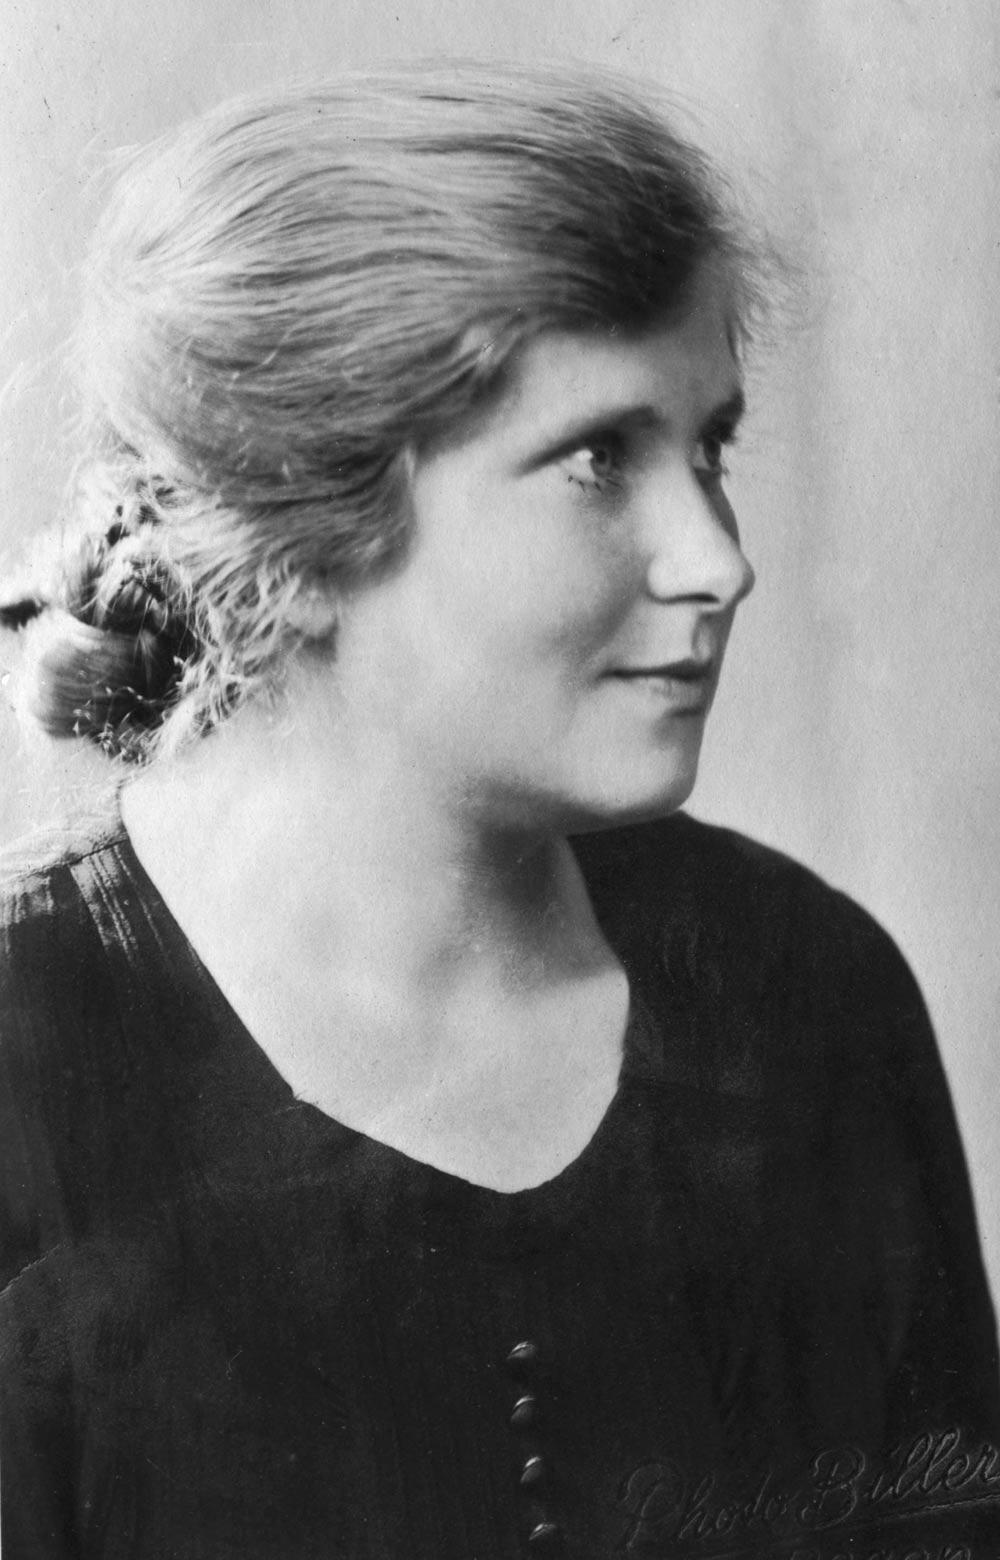
\includegraphics[width=3.413cm,height=5.323cm]{pictures/zulassungsarbeit-img047.jpg}

Abb. \stepcounter{Abb}{\theAbb}: Der „Chor“ der Nachkriegszeit: Mathilde
Glasschröder &

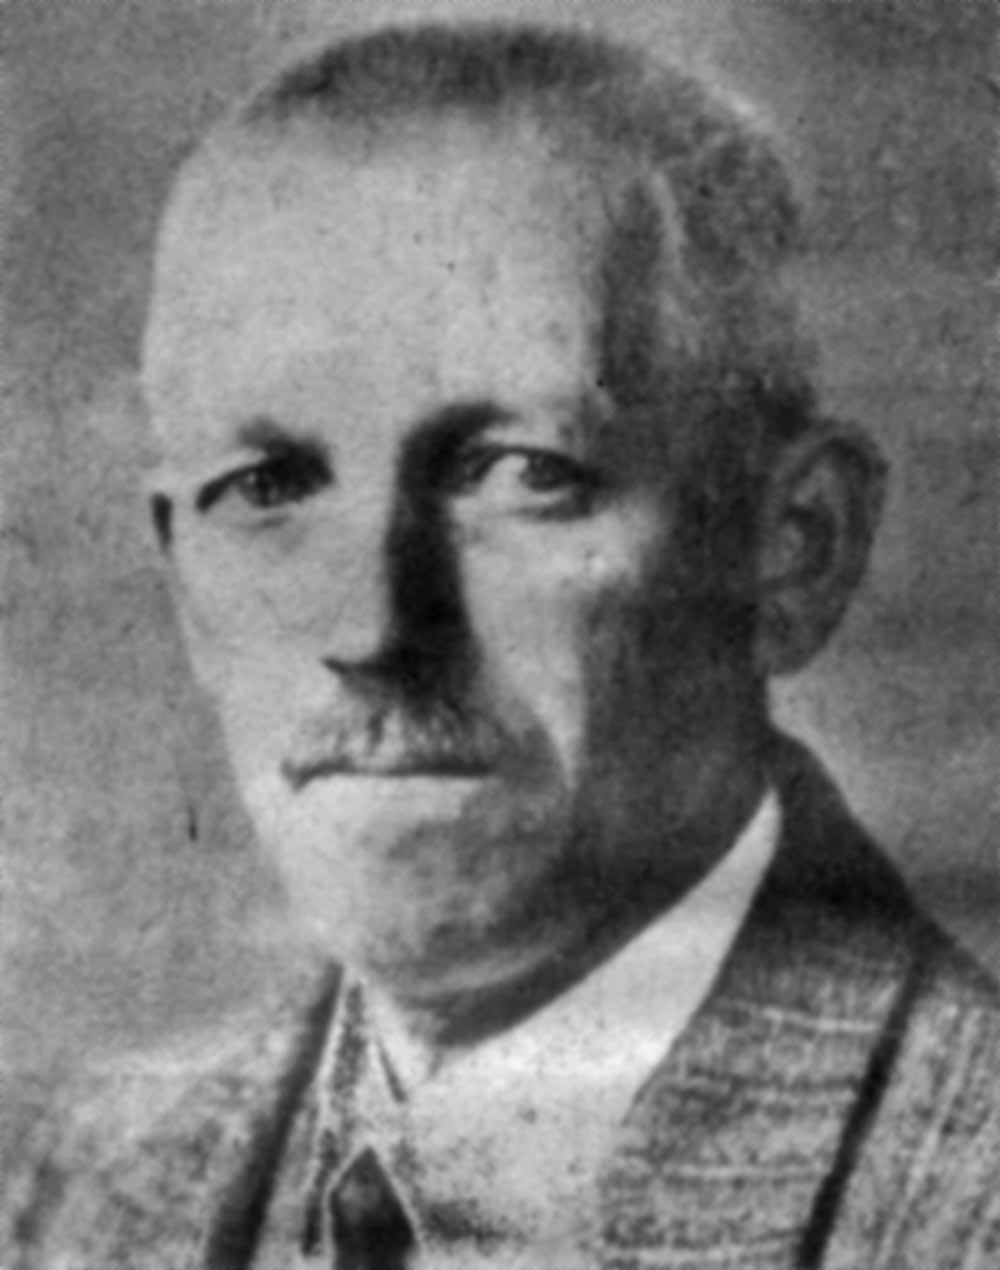
\includegraphics[width=4.18cm,height=5.308cm]{pictures/zulassungsarbeit-img048.jpg}

Abb. \stepcounter{Abb}{\theAbb}: August Högn &

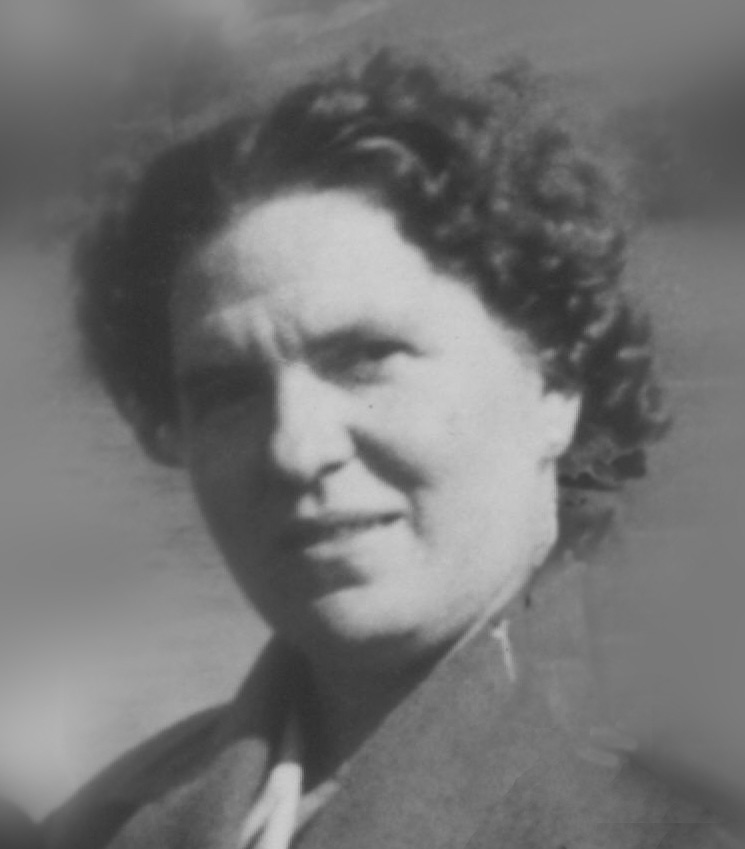
\includegraphics[width=3.942cm,height=5.3cm]{pictures/zulassungsarbeit-img049.jpg}

Abb. \stepcounter{Abb}{\theAbb}: Barbara Essigmann  &

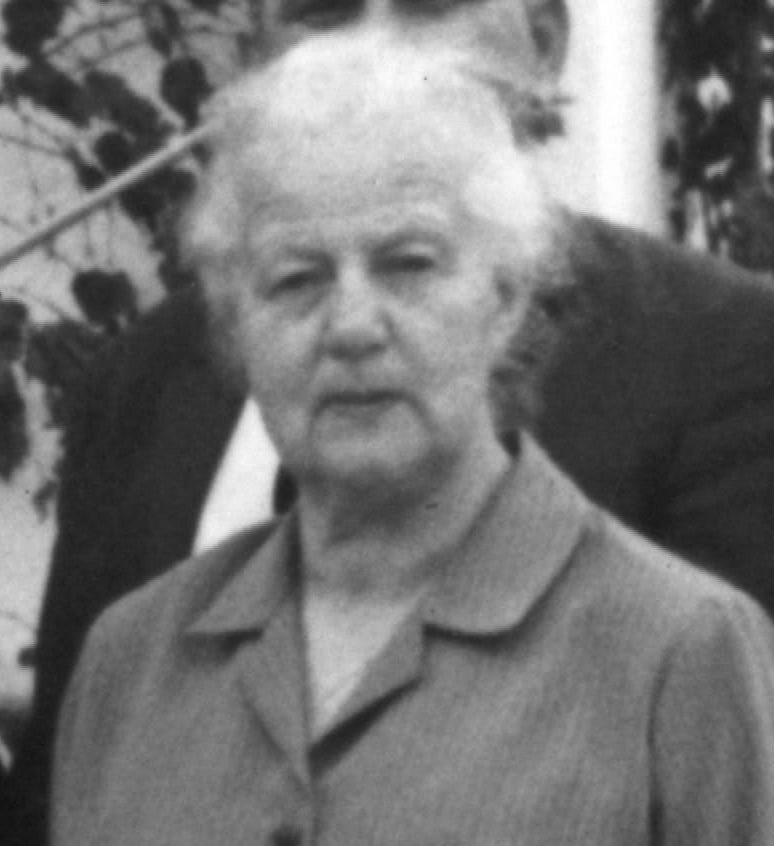
\includegraphics[width=3.194cm,height=5.281cm]{pictures/zulassungsarbeit-img050.jpg}

Abb. \stepcounter{Abb}{\theAbb}: Theres Raster\\
\end{supertabular}
\end{flushleft}
Der „Chor“, der unter der Woche sang, bestand nur aus vier Personen: Den
drei Sängerinnen Mathilde Glasschröder, Barbara Essigmann, Theres
Raster, und August Högn, der selbst eine Männerstimme
übernahm. \footnote{Interview Nr. 24, Johann Glasschröder, 28.12.2004,
Absatz 2} Vor allem die Heterogenität der einzelnen Stimmen
untereinander, die durch die Kleinstbesetzung unverdeckt hervortrat,
hinterließ bei so manchen Kirchenbesuchern einen schlechten
Eindruck. \footnote{Interview Nr. 9, Dr. Doraliesa Wiegmann, 19.1.2003,
Absatz 4; Interview Nr. 24, Johann Glasschröder, 28.12.2004, Absatz 36}
Wurde Mathilde Glasschröder als sängerische Naturbegabung mit großer
Stimme vergleichbar einer Opernsängerin beschrieben,\footnote{
Interview Nr. 13, Lorenz Schlagintweit, 29.11.2003, Absatz 2; Interview
Nr. 24, Johann Glasschröder, 28.12.2004, Absatz 52} blieb Theres Raster
als außerordentlich schlechte Sängerin mit „fürchterlichem“ Stimmklang
in Erinnerung. \footnote{Interview Nr. 24, Johann Glasschröder,
28.12.2004, Absatz 46} Die alternde Stimme Högns scheint sich ebenso
wenig in einen Gesamtklang eingebunden zu haben. \footnote{Interview
Nr. 24, Johann Glasschröder, 28.12.2004, Absatz 36} Neben dem
schlechtem Gesang stellte für Reicheneder möglicherweise das
kirchenmusikalische Repertoire einen Stein des Anstoßens dar. Ein und
dasselbe Lied, das zum Schluss des Gottesdienstes gesungen wurde, hatte
sich als „Standardstück“ eingebürgert \footnote{Interview Nr. 16, Maria
Freisinger, 25.8.2004, Absatz 20} und nicht nur werktags wurden Teile
aus dem Gloria und Credo übersprungen. \footnote{Interview Nr. 24,
Johann Glasschröder, 28.12.2004, Absatz 26; Interview Nr. 2, Barbara
Essigmann, 27.12.2002, Absatz 36; Interview Nr. 16, Maria Freisinger,
25.8.2004, Absatz 14}

Obwohl in Ruhmannsfelden die Bereitschaft zum Singen recht groß war – es
gab neben dem Kirchenchor einen Männerchor und eine weltliche
Liedertafel \footnote{Interview Nr. 24, Johann Glasschröder,
28.12.2004, Absatz 10, 4 } – gab es in Ruhmannsfelden lediglich ein
Gesangsquartett als Kirchenchor. Reicheneder muss als Hauptgrund für
diesen Missstand die laxe Probenpraxis in Högns Wohnung angesehen
haben, den er durch Ansetzung von öffentlichen Proben zu beseitigen
versuchte – wohl bemerkt mit Högn als Chorleiter. \footnote{Interview
Nr. 24, Johann Glasschröder, 28.12.2004, Absatz 43 – 44} Es ist höchst
ungewöhnlich, wenn nicht ein Chorleiter selbst über die Anberaumung der
Chorproben entscheidet. Einerseits wollte Reicheneder durch diese
Maßnahme wahrscheinlich, das Niveau der musikalischen Darbietungen
erhöhen. Andererseits hoffte er doch insgeheim, dass Högn durch diese
Bevormundung abdankt und die Stelle für seine Vertrauensperson Maria
Reisinger frei macht. Die mit Högn sehr eng befreundeten
Chorsängerinnen Mathilde Glasschröder und Barbara Essigmann erschienen
nicht zu den von Reicheneder festgesetzten Proben \footnote{Interview
Nr. 24, Johann Glasschröder, 28.12.2004, Absatz 42} und lieferten somit
Reicheneder einen Grund zum Einschreiten.

In seinen Briefen an beide Chorsängerinnen und in diesem Fall auch an
Högn teilte Reicheneder allen drei kurz vor Weihnachten 1953 ihre
„Kündigung“ mit. Soweit der Inhalt der Briefe aus Augenzeugenberichten
erahnt werden kann, war zwar in ihnen kein Wort von „Kündigung“ zu
lesen, da aber Reicheneder den Sängerinnen und Högn die Chorabrechnung
beifügte und ihnen für ihre Dienste an der Pfarrkirche Ruhmannsfelden
dankte, machte er ihnen unmissverständlich deutlich, dass er für sie
keinen weiteren Einsatz in der Kirchenmusik vorsah. \footnote{Interview
Nr. 24, Johann Glasschröder, 28.12.2004, Absatz 38 – 40} Diese
„Kündigungsschreiben“ verursachten bei den Betroffenen große
Verärgerung. Als Högn seinen Brief den zwei Sängerinnen zeigte, soll er
Reicheneder sogar als \zitat{„Lackel“} bezeichnete
haben. \footnote{Interview Nr. 2, Barbara Essigmann, 27.12.2002, Absatz
64} Die Verärgerung der Sängerinnen schlug in Hass auf Reicheneder
um, \footnote{Interview Nr. 2, Barbara Essigmann, 27.12.2002, Absatz
16} nachdem wenig später „ihr Högn“ einen schweren Schlaganfall erlitt,
der eine linksseitige Lähmung zur Folge hatte, \footnote{Dokument Nr.
73, Brief von August Högn an Stephan Leitner, 10.3.1961} und in ein
Krankenhaus gebracht werden musste. \footnote{Interview Nr. 24, Johann
Glasschröder, 28.12.2004, Absatz 36} Beide Sängerinnen gaben
Reicheneder die Mitschuld an Högns Schlaganfall. Ein Foto von 1961
zeigt auch deutlich, dass Högn an einer leichten Gesichtslähmung als
Spätfolge des Schlaganfalls litt, und Zeitzeugen berichten von
Beeinträchtigungen beim Sprechen. \footnote{Interview Nr. 2, Barbara
Essigmann, 27.12.2002, Absatz 36} Nur mit Zuhilfenahme eines
Stocks \footnote{Foto bei der Einweihung des Schulanbaus, 7.5.1959}
konnte Högn seitdem gehen. \footnote{Interview Nr. 2, Barbara
Essigmann, 27.12.2002, Absatz 38, 62, 64} An Orgelspielen war nicht
mehr zu denken.

\begin{center}
\begin{minipage}{10.084cm}
\begin{flushleft}
\tablefirsthead{}
\tablehead{}
\tabletail{}
\tablelasttail{}
\begin{supertabular}{m{5.018cm}m{4.6670003cm}}

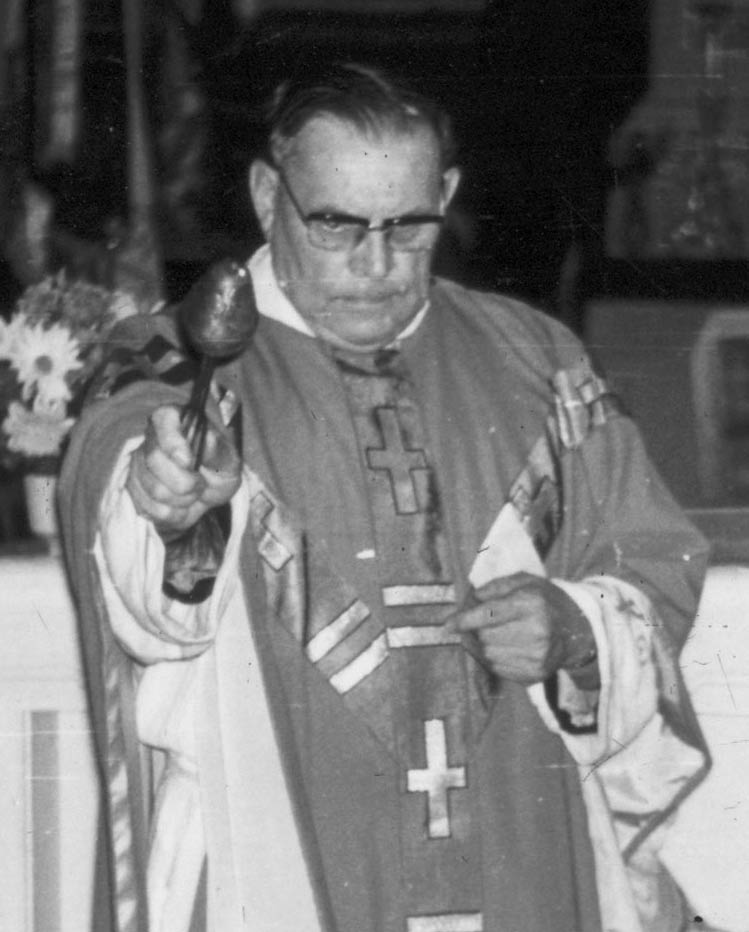
\includegraphics[width=4.835cm,height=5.992cm]{pictures/zulassungsarbeit-img051.jpg}

Abb. \stepcounter{Abb}{\theAbb}: Franz Seraph Reicheneder &

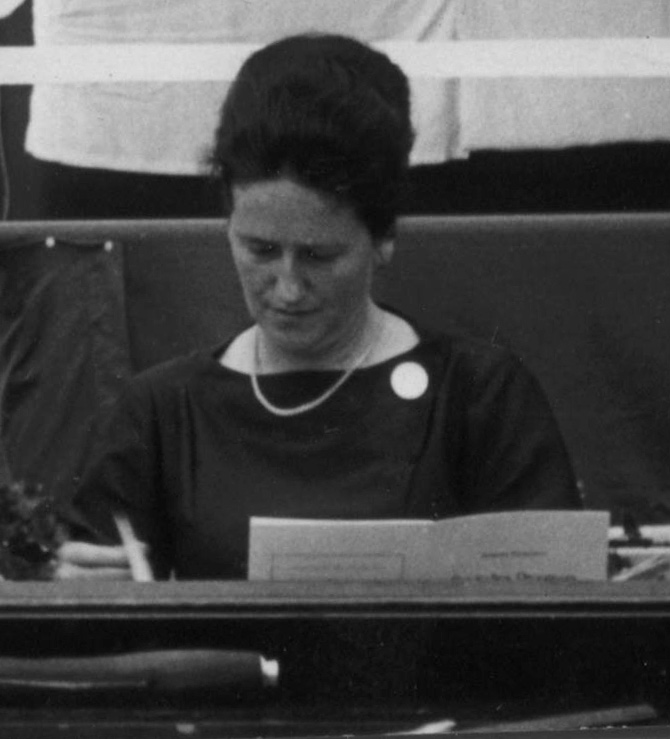
\includegraphics[width=4.484cm,height=6.003cm]{pictures/zulassungsarbeit-img052.jpg}

Abb. \stepcounter{Abb}{\theAbb}: Maria Reisinger\\
\end{supertabular}
\end{flushleft}
\end{minipage}
\end{center}
Deshalb wirkt der Brief, den Högn nach seinem Krankenhausaufenthalt am
25.1.1954 an Reicheneder schrieb, schon etwas befremdlich. Mit der
\zitat{„berechtigten Forderung auf Ruhestand auch im
Kirchenchordienst“} verkündete Högn in diesem Schreiben seinen
Rücktritt als Chorregent und Organist und bezog sich dabei nicht auf
die Folgen seines Schlaganfalls oder auf das „Kündigungsschreiben.“
 \footnote{Dokument Nr. 18, Brief von August Högn an Pfarrer
Reicheneder, 25.1.1954} In seinem Antwort-Brief vom 6.2.1954 nahm
Reicheneder zu Högns erhaltenen Brief Stellung, in dem Högn von sich
aus abdankte, und unterstrich, dass er Högns
\zitat{„Standpunkt voll und ganz verstehen“} könne, seinen
Rücktritt aber \zitat{„sehr bedauere.“ } \footnote{Dokument
Nr. 19, Brief von Pfarrer Reicheneder an August Högn, 6.2.1954}

Wären nur diese zwei Briefe und nicht zusätzlich die genauen
Erinnerungen von mehreren Zeitzeugen zur Verfügung gestanden, hätte man
eine ganz andere Schlussfolgerung daraus gezogen. Sowohl Reicheneder
als auch Högn waren daran interessiert, der Nachwelt eine andere
Version des Ausscheidens Högns als die der Kündigung durch Reicheneder
zu überlassen. Nur zwischen den Zeilen, kann man in beiden Briefen die
vorhergehenden Ereignisse erahnen, wie zum Beispiel an der Stelle, an
der Högn die \zitat{„Kündigung seitens des Hochwürdigen Herr
Pfarrers und der gleichen“} als \zitat{„blödes
Weibergeschwätz“} bewertet und darauf hinweist, dass
\zitat{„eine vertragliche Abmachung über den
Kirchenchordienst zwischen Pfarramt Ruhmannsfelden“ }und ihm niemals
bestanden hätte.“  \footnote{Dokument Nr. 18, Brief von August Högn an
Pfarrer Reicheneder, 25.1.1954}\zitat{ }Und seine angebliche
\zitat{„Stimmbandlähmung“,} \footnote{Dokument Nr. 19, Brief
von Pfarrer Reicheneder an August Högn, 6.2.1954}\zitat{ }die
Reicheneder als Entschuldigung anführte, weshalb er Högn keinen
Krankenbesuch abstattete, erscheint in diesem Zusammenhang mehr als
eine faule Ausrede.

Über den wahren Wortlaut der „Kündigungsbriefe“ ließe sich natürlich
viel spekulieren. Allein schon ihr Verschwinden ist ein Beweis für ihre
Brisanz. Reicheneder war ein passionierter Historiker und Archivar. Es
gibt wohl keinen auf die hiesige Gegend bezogenen Zeitungsartikel aus
Reicheneders Ruhmannsfeldener Zeit, der nicht in seine über 30 prall
gefüllte Ordner umfassende „Chronik Ruhmannsfelden“ angefügt wurde.
Auch seine Korrespondenz dokumentierte Reicheneder sehr genau. Viele
von ihm verfasste Briefe lassen sich im Pfarrarchiv im
Kohlepapierabdruck nachlesen, wie etwa das Schreiben an Högn vom
6.2.1954. Die „Kündigungsschreiben“ hat Reicheneder ganz bewusst nicht
archiviert, damit kein schlechtes Licht auf ihn fällt. Einen kaum
unwürdigeren Abschied hätte Reicheneder Högn nach 43 Jahren Dienstzeit
an der Kirchenmusik in Ruhmannsfelden nicht bieten können.

Diese ungerechte Vorgehensweise von Reicheneder gegenüber Högn ist kein
Einzelfall. Ein Ereignis wenige Jahre später ist bezeichnend für
Reicheneders Problemlösungsstrategie mit der „Brechstange“: Nachdem
Pfarrer Reicheneder bei einer Sonntags-Predigt von der Kanzel aus unter
anderem über die \zitat{„Leistungsabzeichen für nächtliche
Liebesfahrten“} \footnote{
http://home.vrweb.de/pfarrei.ruhmannsfelden/reichene.htm} wetterte, die
am Fußballer Ball 1957 verliehen wurden, ließen sich die Beschuldigten
nicht zurechtweisen und veranstalten, nach Angaben des Geistlichen
selbst, aus einer Trotzreaktion heraus ein Faschingsbegräbnis am
Aschermittwoch mit Musik und Saufgelage. \zitat{„Bis die
Haupträdelsführer beim Pfarramt vorstellig geworden sind“;}\footnote{
http://home.vrweb.de/pfarrei.ruhmannsfelden/reichene.htm} wie es in
einer Pressemitteilung des Pfarramts hieß, sollten nun die Glocken in
Ruhmannsfelden schweigen. Diese Aktion machte natürlich nicht nur in
der regionalen Presse ihre Runde. Die Glocken läuteten erst wieder, als
sich der Bürgermeister von Ruhmannsfelden in den Fall einbezog und für
eine Lösung des Problemfalls sorgte, die schriftlich festgehalten
wurde.\footnote{
http://home.vrweb.de/pfarrei.ruhmannsfelden/reichene.htm}

In der Kirchenverwaltungssitzung vom 21.2.1954 wurde Högns Nachfolge
endgültig geregelt. Maria Reisinger erhielt die Organistenstelle und
Franz Danziger übernahm die Chorleitung. \footnote{Dokument Nr. 124,
Protokoll der Kirchenverwaltungssitzung, 21.2.1954}
